\chapter{Design}
Now we will design how to implement what we have defined in the analysis chapter.
Our application is a single-page web application.

\section{Architecture}
\begin{figure}[h]
  \centering
  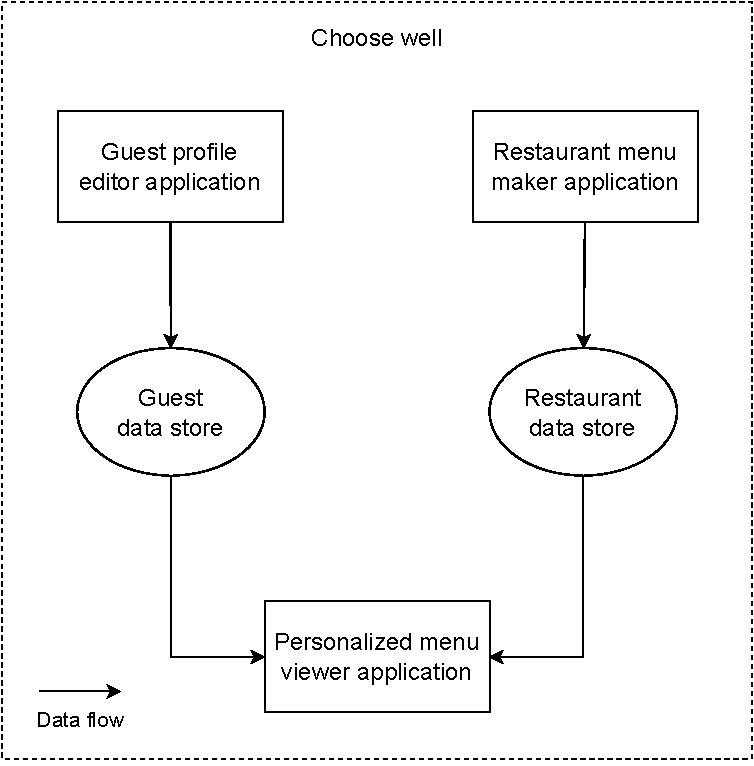
\includegraphics[width=0.62\linewidth]{master-thesis/img/architecture_data_flow.pdf}
  \caption{Application's data flow diagram}
\end{figure}

\section{Technological stack}
There are various options out there for what technologies we can use to implement our application.
This section contains an overview of available tools and which ones we chose and why.

\subsection{User interface}
Nowadays, there are many frameworks for building web applications.
We need to be able to create an interactive user interface.
We need to have state for logged in user.
We need to fetch data from the internet.
We need to integrate with Solid.
The most popular are listed below with their pros and cons.

\subsection*{Considered technologies}
Angular, React, Vue

\subsubsection*{Angular}
Angular is a platform and framework for building single-page client applications using HTML and TypeScript. 
It implements its core and optional functionality as a set of TypeScript libraries. 
The basic building blocks of the Angular framework are Angular components that are organized into \emph{NgModules}. 
NgModules collect related code into functional sets; an Angular application is defined by a set of NgModules.

\subsubsection*{React.js}
React is a JavaScript library for rendering user interfaces.
Applications written in React are built from modular and reusable pieces called components.
React components receive data and return what should appear on the screen. 
They can be passed new data in response to an interaction, like when the user types into an input. 
React will then update the screen to match the new data.
A notable feature is the use of a virtual Document Object Model, or Virtual DOM. 
React creates an in-memory data-structure cache, computes the resulting differences on a re-render, and then updates the browser's displayed DOM efficiently. 
This selective rendering provides a major performance boost.

\subsubsection*{Vue.js}
Vue is a JavaScript framework for building user interfaces. 
It builds on top of standard HTML, CSS, and JavaScript and provides a declarative and component-based programming model.
Vue uses an HTML-based template syntax that allows programmers to declaratively bind the rendered DOM to the underlying component instance's data.
Under the hood, Vue compiles the templates into highly-optimized JavaScript code. 
Combined with the reactivity system, Vue can intelligently figure out the minimal number of components to re-render and apply the minimal amount of DOM manipulations when the app state changes.

\subsection*{Chosen technology}


\subsection{nasadenie}
%  Vite
% alternatives: create react app, webpack

\subsection{client-side routing}
% react router if used

\subsection{Programming language}
As for programming languages, we considered two options. 

\subsection*{Considered technologies}
JS, TS

\subsubsection*{JavaScript}
JavaScript is a lightweight, interpreted, or just-in-time compiled programming language with first-class functions. 
It is most well-known as the scripting language for Web pages. 
JavaScript is a prototype-based, multi-paradigm, single-threaded, dynamic language, supporting object-oriented, imperative, and declarative---e.g. functional programming styles.

\subsubsection*{TypeScript}
TypeScript is a superset of JavaScript. 
It provides features such as optional static typing, classes, interfaces, and generics. 
The goal of TypeScript is to help catch mistakes early through its type system and make JavaScript development more efficient. 
One of the big benefits is enabling IDEs to provide a richer environment for spotting common errors as the programmer types their code.

\subsection*{Chosen technology}


\subsection{balickovaci nastroj}
%  npm 
% alternatives: yarn
\subsection*{Considered technologies}

\subsubsection*{}

\subsubsection*{}

\subsection*{Chosen technology}

\subsection{Responsive design}
We need our application to be responsive to various device screens.

\subsection*{Considered technologies}
Bootstrap, MUI
\subsubsection*{Bootstrap}

\subsubsection*{Material UI}

\subsection*{Chosen technology}



\subsection{Persistence}
We need to store and later read data.
% Solid pods
\subsection*{Considered technologies}

\subsubsection*{}

\subsubsection*{}

\subsection*{Chosen technology}

\subsection{Testing}
We need to test our application in order to prevent bugs during implementation.
% https://legacy.reactjs.org/docs/testing-environments.html
\subsection*{Considered technologies}

\subsubsection*{}

\subsubsection*{}

\subsection*{Chosen technology}

\subsection{Documentation}
We need to capture how our application works for users and future developers.
% (GitHub markdown)
\subsection*{Considered technologies}

\subsubsection*{}

\subsubsection*{}

\subsection*{Chosen technology}
